\setcounter{chapter}{-1}
%\chapter{Interface}
%\addcontentsline{toc}{chapter}{Interface}

\lab{Algorithms}{Interface Introduction}{Interface Introduction}
\objective{This lab will teach how to navigate the MATLAB interface, IO, and help. It can be skipped by users familiar with MATLAB.}

Computation is the muscle of applied mathematics. Regardless of the field of study, inevitably there is a need to utilize computers to answer real world questions. MATLAB (which stands for matrix laboratory) is the program that we use in this text to answer these questions. MATLAB is a powerful tool, which allows us to answer a wide variety of questions computationally. MATLAB can be overwhelming at first, which is why we offer a user-friendly introduction to the MATLAB interface. %When you first launch MATLAB you may feel a little overwhelmed by all the windows and options that are in front of you.  The interface is also very customizable, so even an experienced user may be a little disoriented when the application first launches before they catch their bearings.

\section*{Getting Started} When first launched, MATLAB may seem overwhelming.  There are many options and menus presented by a highly customizable interface (see figure 1).  Even experienced users can be disoriented when the application launches before they catch their bearings.

The first thing to note is the command window.  This is essentially a command prompt that allows us to execute commands, navigate the file structure, and run programs.  

\begin{figure}[h!]
\begin{center}
	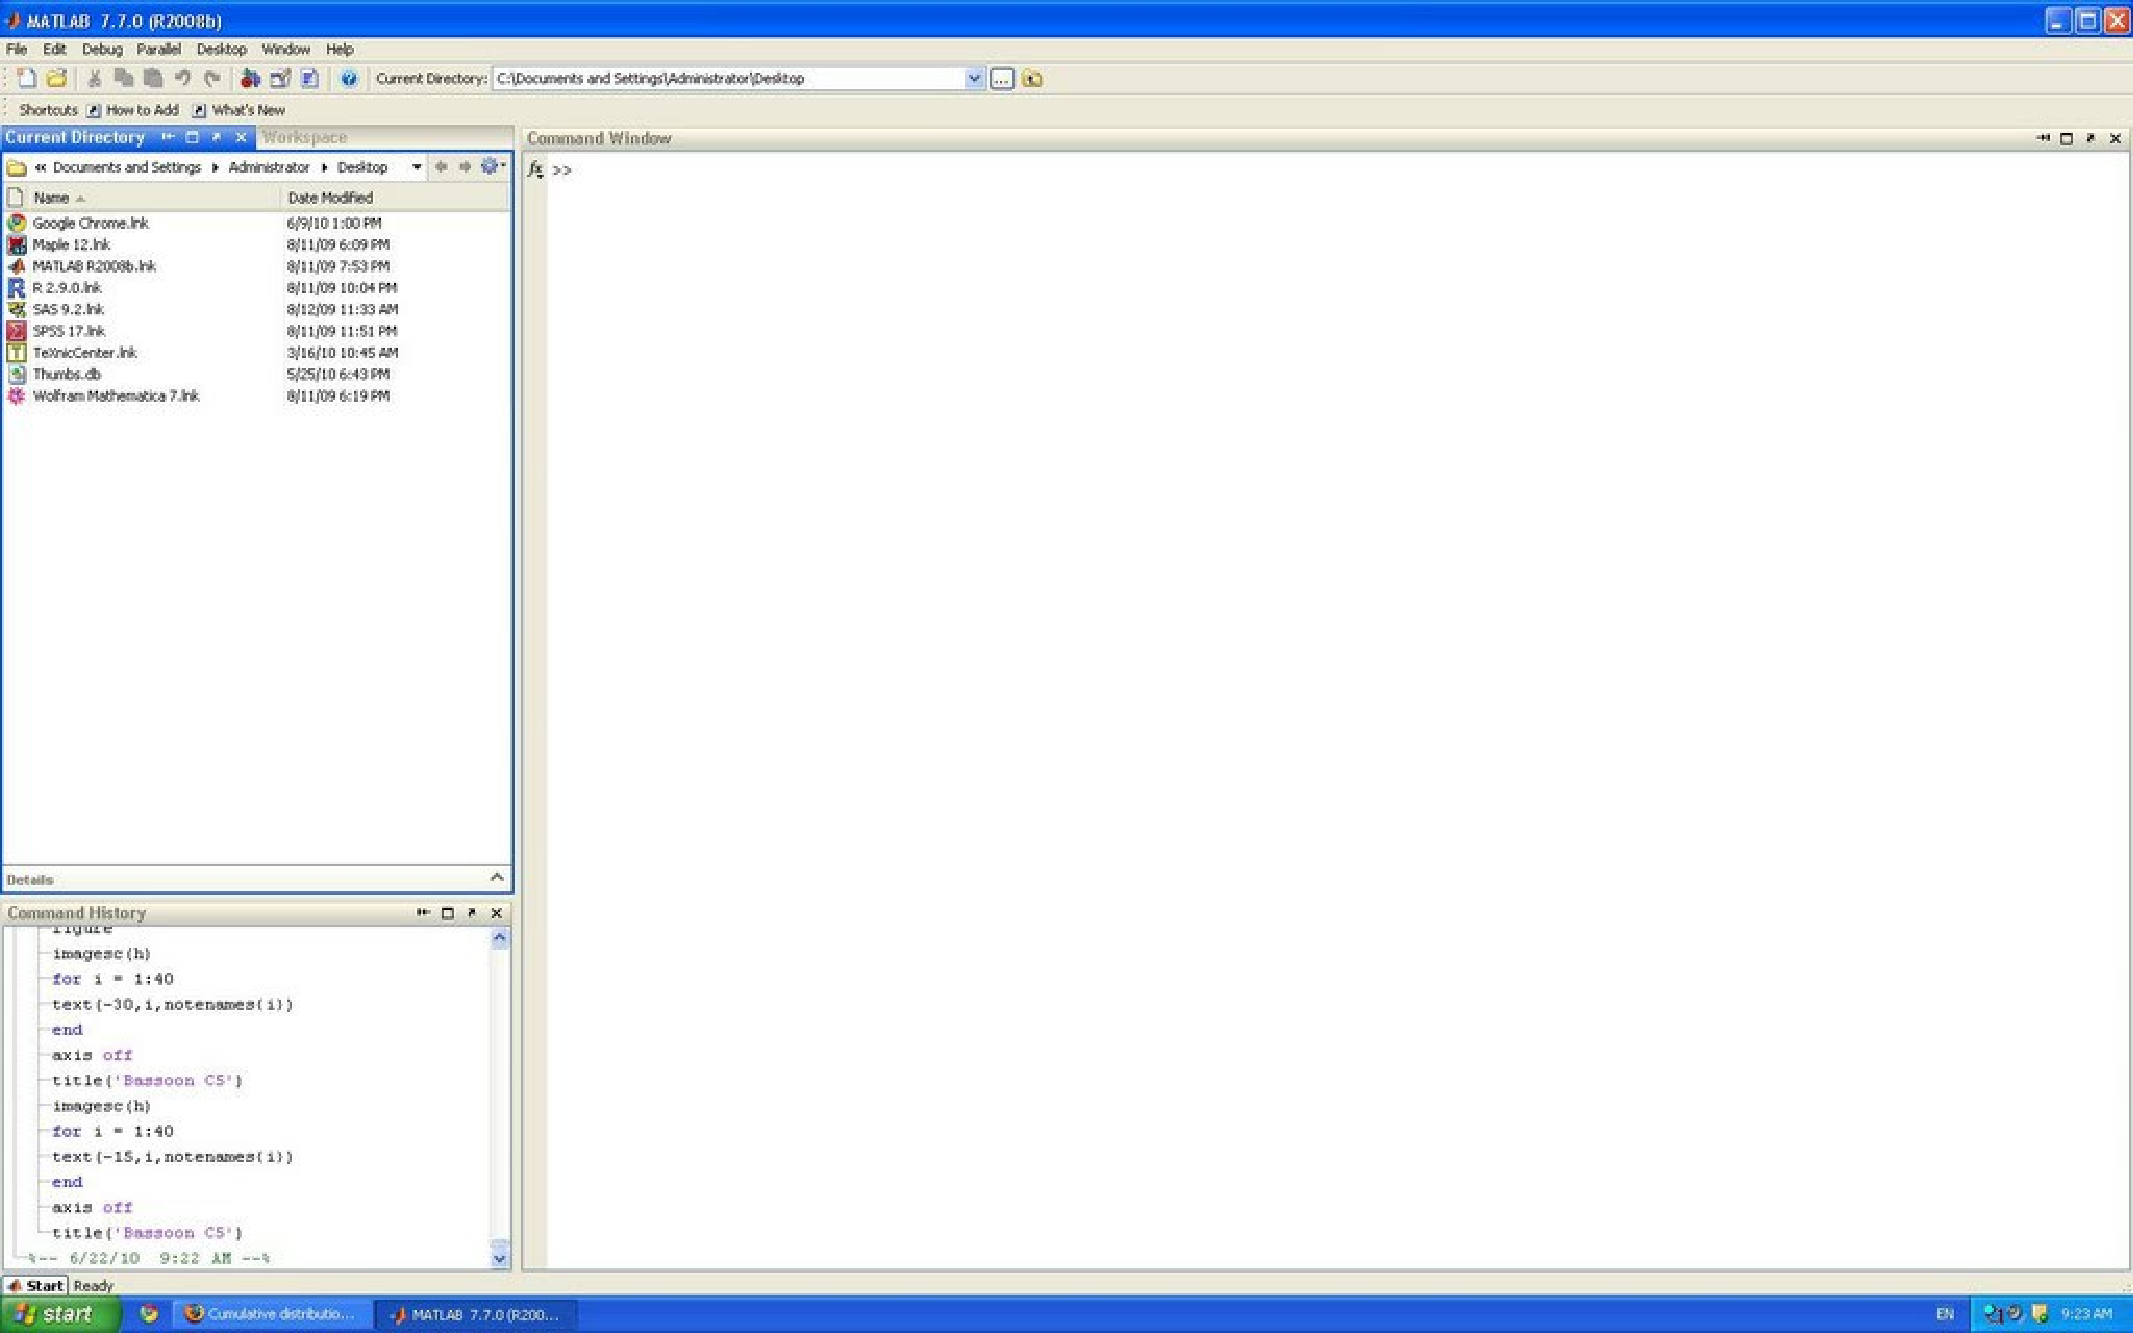
\includegraphics[scale=0.3]{./Figures/homeScreen}
	\caption{The startup screen for MATLAB. The command window is the largest portion of the screen}
\end{center}
\end{figure}


MATLAB is an interpreted language, which means that we can immediately begin executing commands without compiling.  For example, if you type 1 + 1 at the $>>$ prompt in the command window, MATLAB will immediately return the answer. Figure 2 represents basic arithmetic operations we can perform in MATLAB commands:

\begin{figure}[h!]
\begin{center}
	\begin{tabular}{|c|c|}
	\hline
	\li{+} & Addition \\
	\li{-} & Subtraction \\
	\li{*} & Multiplication \\
	\li{/} & Division \\
	\hline
	\end{tabular}
	\caption{Simple Arithmetic Operators}
\end{center}
\end{figure}

\begin{lstlisting}[style=matlab]
>> 1 + 1
ans =
     2
\end{lstlisting}


Now notice the Current Directory panel in figure 1.  Just like a DOS prompt, MATLAB can only see files that are in its current directory and its customizable path.  You can navigate the file structure using the interface in the Current Directory panel, or you may use \li{cd}, \li{dir}, and \li{what} in the command window.  For example:

\begin{lstlisting}[style=matlab]
>> dir
.                            CS312                        ORCA.doc                                    
..                           IMPACT Presentations         ORCA.pdf                       
.DS_Store                    Linearalgebra (1).pdf        PDEs                           
>> cd MATLAB
>> what
M-files in the current directory /Users/jaredwebb/Documents/MATLAB
HelloWorld         coinText           graphscript        outLierRemove      
adjustSet          compareImages      imageReducer       reconSignal        
bigSignal          fourierCompare     littleSignal       sigScript          
coinTest           generateGraphs     myfft              sigTest            
\end{lstlisting}

Note that the \li{what} command lists the m-files in the current directory. M-files are files that contain MATLAB commands.  We discuss M-files in further details in Chapter 1.

\begin{problem}
Create a new text file containing only the string of numbers \li{1 2 3 4 5} and call it \li{data.txt}.  Using the command window, navigate to the location of the file then type \li{load data.txt}.  What happens?
\end{problem}

Also note the Command History and the Workspace panes.  The command history will show all the commands that you have issued in the command window.  You can also access these by using the up or down arrow to cycle through your Command History.  The workspace pane shows all of the current variables that MATLAB is storing.  The \li{who} command will print your workspace to the command line.

\begin{lstlisting}[style=matlab]
>> who
Your variables are:
ans
\end{lstlisting}

\section*{Getting Help}

Even the most experienced MATLAB programmer will run into commands they do not recognize or do not remember how to solve.  In fact, the mark of an experienced programmer is not so much knowing automatically how to use every single MATLAB command as much as it is knowing what resources are available and how to quickly distill those resources into useful commands for the specific problem.

The \li{help} and \li{doc} commands allow you to access the MATLAB documentation about a specific command.  The \li{help} command will give you a detailed plaintext explanation of a command and its parameters, while \li{doc} will bring up details in a browser along with pictures and examples.

When \li{help} and \li{doc} fail there are many resources online that are extremely helpful, especially when dealing with specific problems.  MATLAB is indeed the language of technical computing, and there is an active community of researchers that will have run into and solved myriad problems.  %When in doubt, google.


\begin{center}
\begin{figure}
	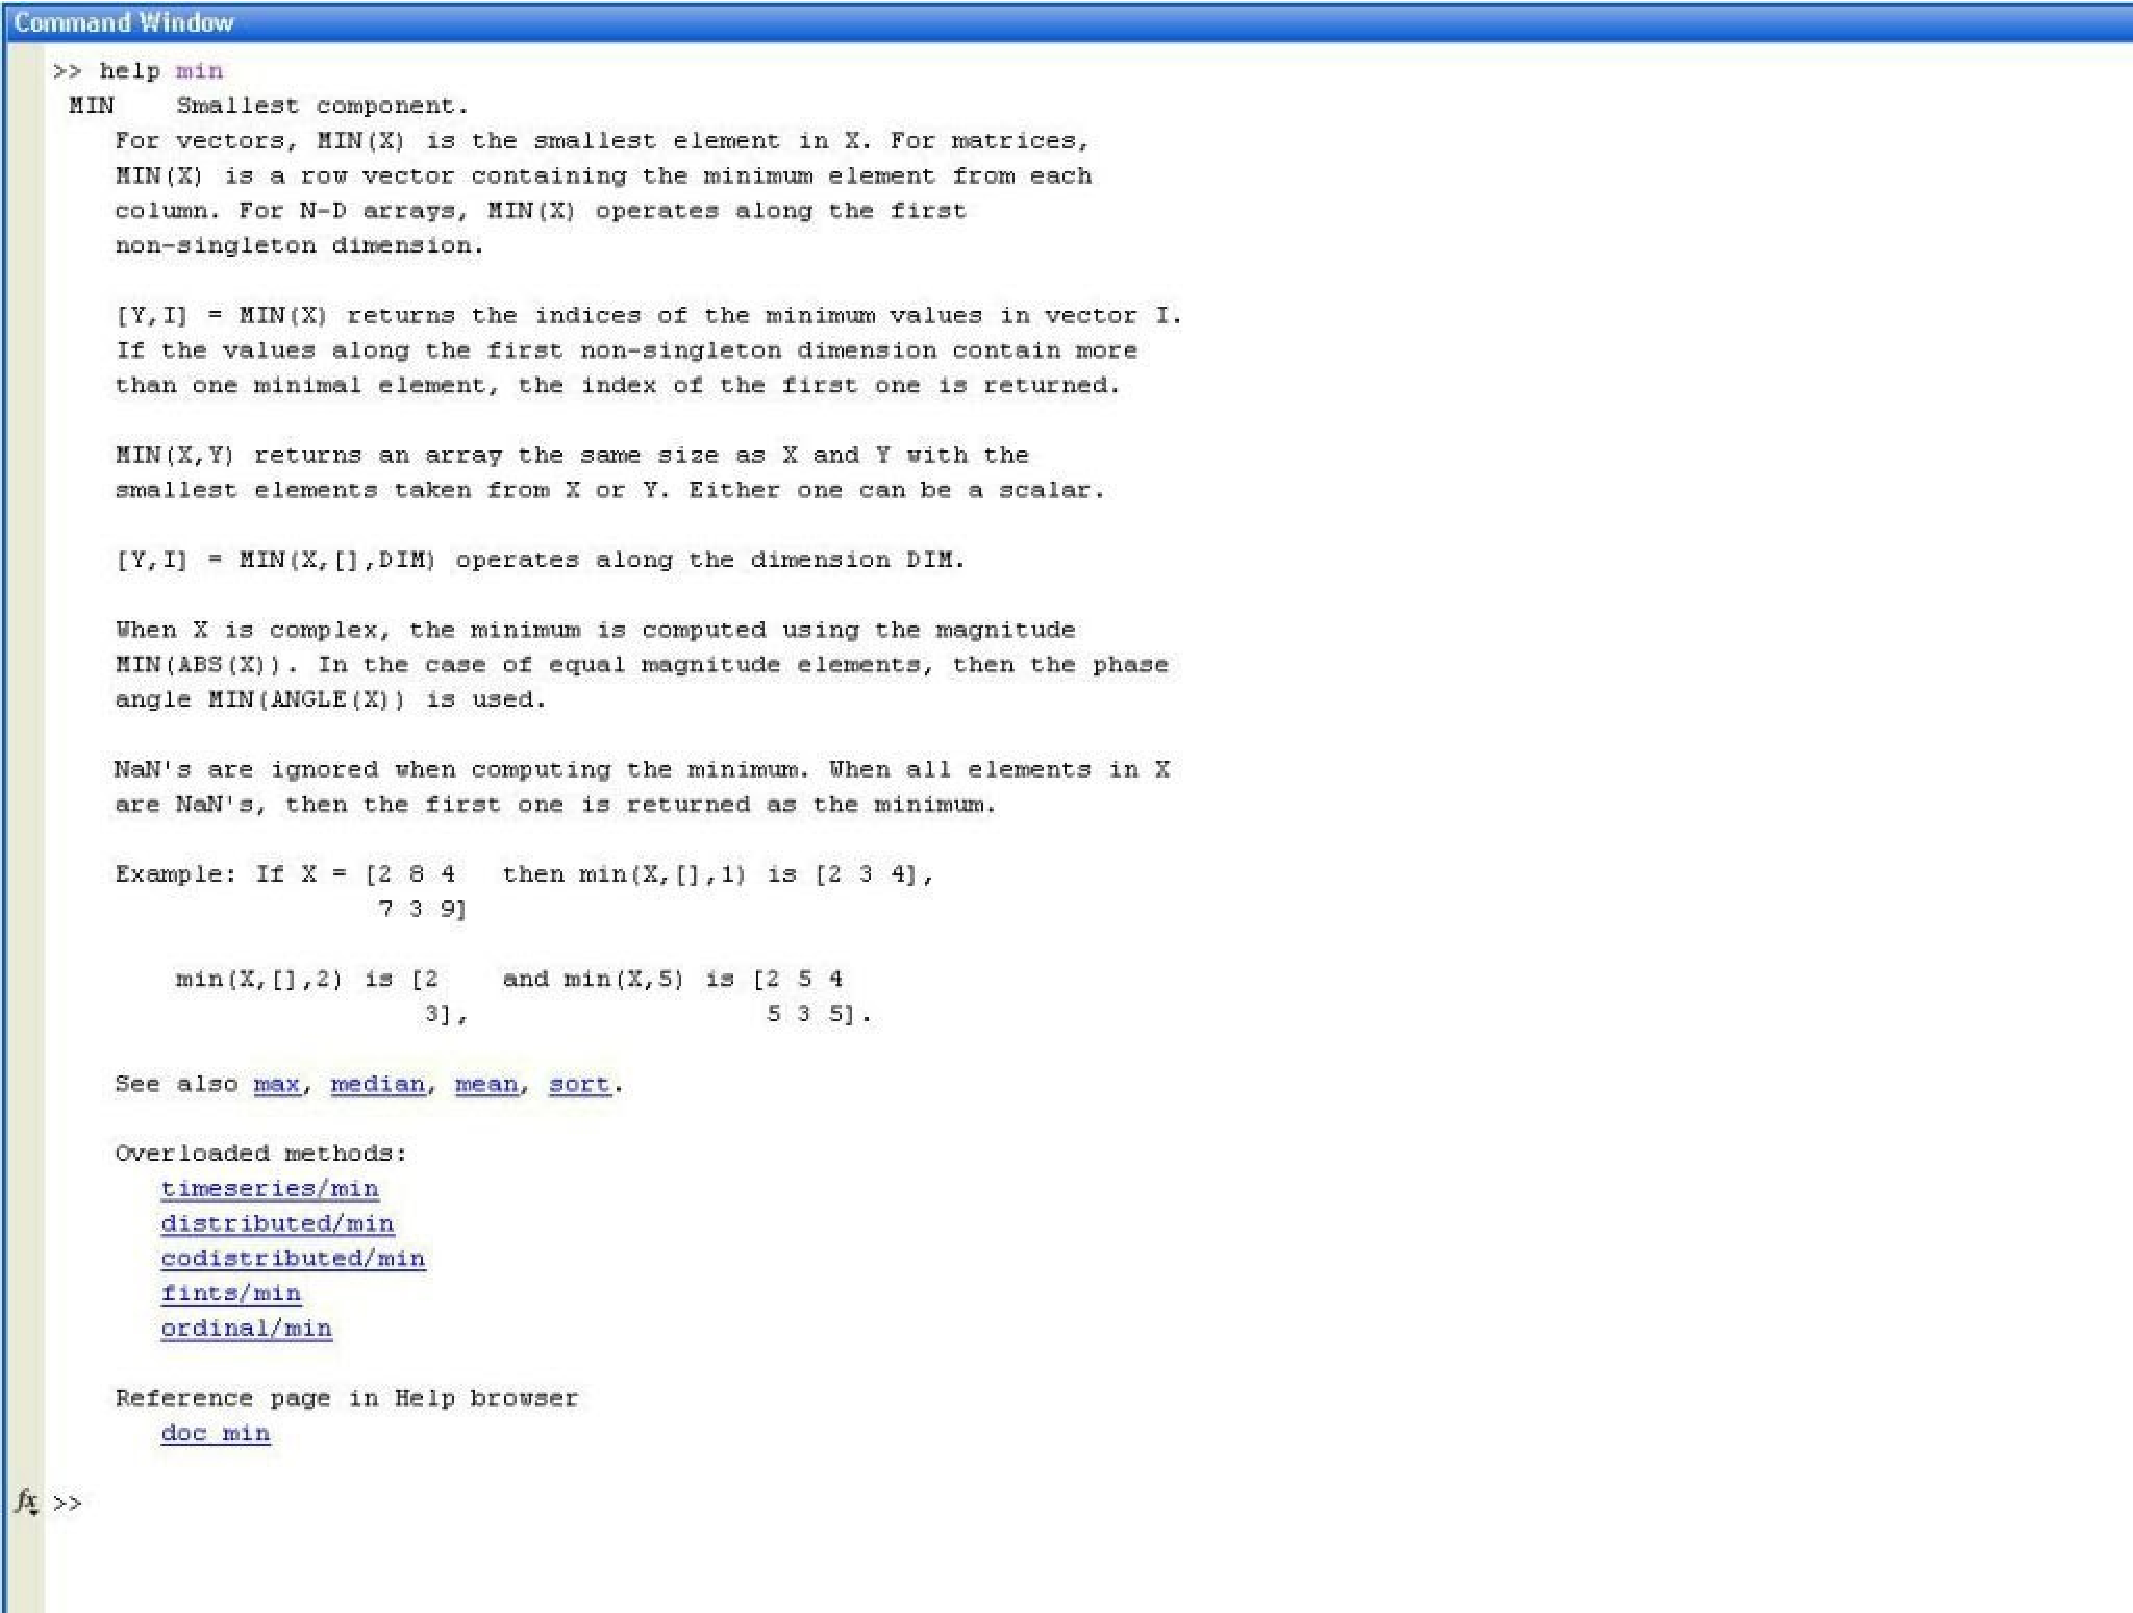
\includegraphics[scale=0.3]{./Figures/help}
	\caption{The help documentation for the \li{min} command. Note that the information displays in the command window.}
\end{figure}
\begin{figure}
	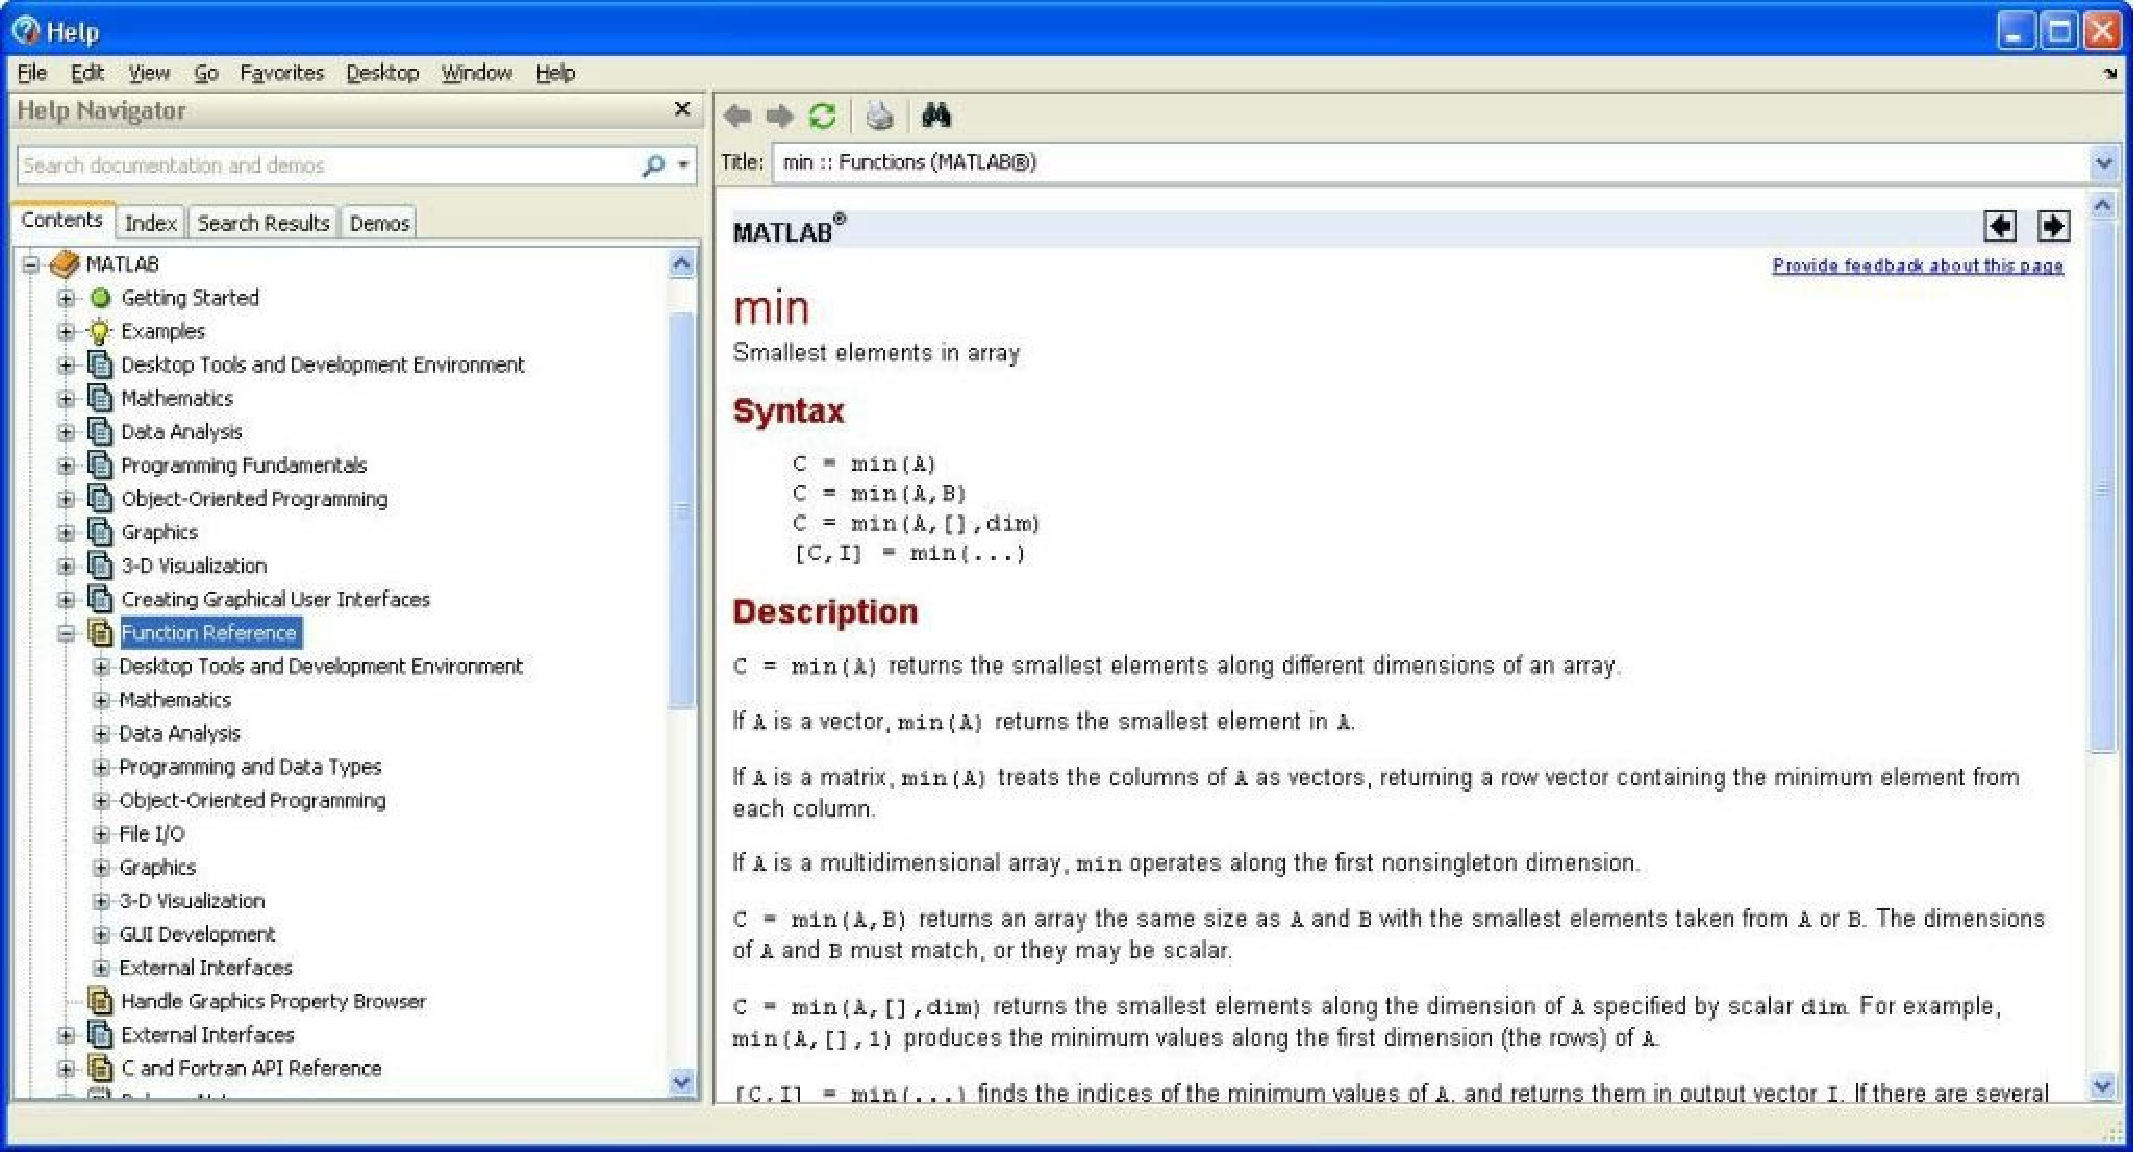
\includegraphics[scale = .3]{./Figures/doc}
	\caption{The documentation window for the \li{min} command. This can be accessed by typing \li{doc min} at the command line.}
\end{figure}
\end{center}

\begin{problem}

Using MATLAB's built in documentation, identify the function of the following commands
\begin{itemize}
	\item fzero
	\item find
	\item linprog
\end{itemize}
\end{problem}

\begin{problem}

Use MATLAB's built in documentation to do the following

\begin{itemize}
	\item Find the zeros of $x^2 - 3x + 2$
	\item Generate a vector of 5 random numbers from a Poisson distribution
	\item Calculate 25 choose 10
\end{itemize}	

\end{problem}

\section*{Setting Variables}

Setting variables in MATLAB happens just as you would expect, using \li{=} to assign a value to a letter or string.

\begin{lstlisting}[style=matlab]
>> x = 3
x =
     3
>> my_variable = 2
my_variable =
     2
>> x + my_variable
ans =
     5
\end{lstlisting}

Placing a semicolon on the end of a MATLAB expression will suppress output.

\begin{lstlisting}[style=matlab]
>> x = 3;
>> my_variable = 2;
>> x + my_variable
ans =
     5
\end{lstlisting}

MATLAB supports several datatypes.  As you become more experienced you will become acquainted with the subtleties of using a specific data type.  We only list them here, noting that in MATLAB the default data type is double.

\begin{figure}[h!]
\begin{center}
	\begin{tabular}{|c|c|}
	\hline
	Class Name & Usage \\
	\hline
	\li{single} & single precision floating point\\
	\hline
	\li{double} & double precision floating point\\
	\hline
	\li{(u)int8} & (un)signed 8 bit integer\\
	\li{(u)int16} & (un)signed 16 bit integer\\
	\li{(u)int32} & (un)signed 32 bit integer\\
	\li{(u)int64} & (un)signed 64 bit integer\\
	\hline
	\li{char} & characters and strings\\
	\hline
	\li{logical} & boolean values\\
	\hline
	\end{tabular}
\end{center}
\caption{Data types in MATLAB}
\end{figure}

\section*{Saving A Workspace}

Large projects can include many variables.  MATLAB allows us to save the entire workspace to a file that can be re-imported.

%Example inserted here%

\begin{figure}
\begin{center}
	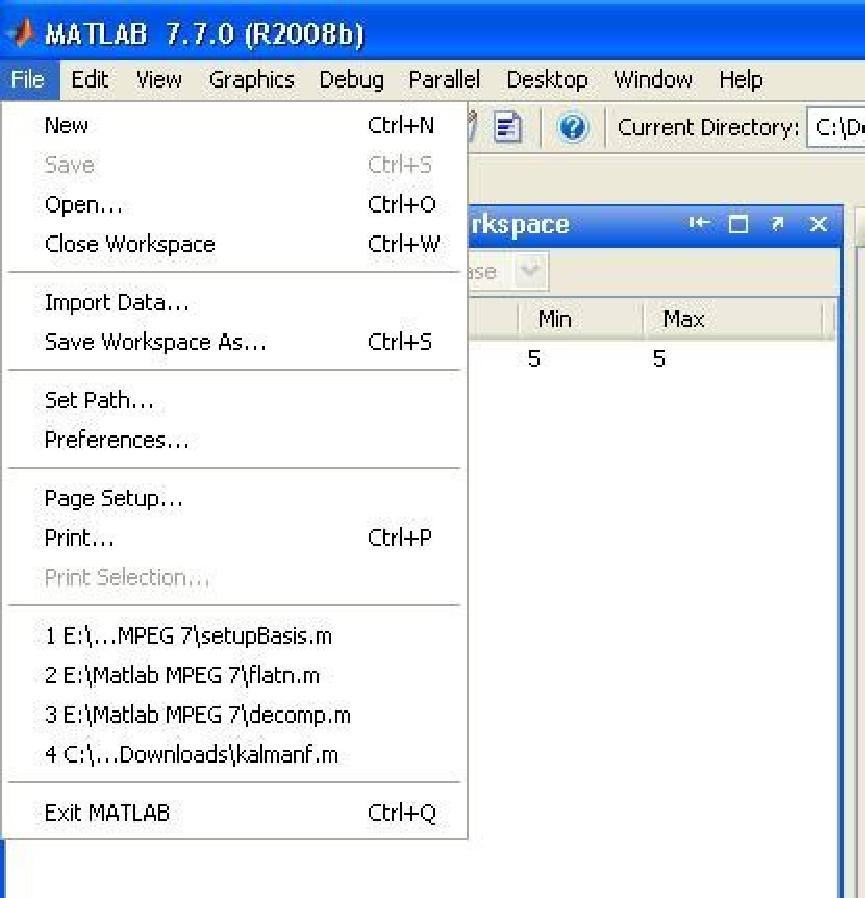
\includegraphics[scale=0.5]{./Figures/saveWorkspace}
	\caption{The file menu. Note the option to save the workspace.}
\end{center}
\end{figure}

\section*{A Note on Floating Point Arithmetic}

In mathematics we expect that the difference between two equal quantities to be zero.  For example, $10 - 10 = 0$.  floating point arithmetic isn't always so precise - altering the previous expression to $e^{log(10)} - 10 = 0$ changes nothing on paper, but try putting it into MATLAB:

\begin{lstlisting}[style=matlab]
>> 10 - 10
ans =
     0
>> exp(log(10)) - 10
ans =
   1.7764e-15
\end{lstlisting}

This is due to floating point arithmetic. Floating point numbers do not have arbitrary precision: they only occupy a certain amount of memory.  For numbers with long decimal expressions or irrational numbers, there will inevitably be a loss of precision because of this memory constraint.  Although these errors will generally be small it is important to understand this limitation of numerical computation. The intricacies of floating point arithmetic will be further developed in Volume II of this work.
